In the world of marine and underwater robotics, we can identify two categories of elements: mobile marine objects (MMO) and flexible tethers (FT)~\cite{blintsov_development_2017}. Mobile marine objects include surface vessels, submarines, and remotely operated vehicles~\cite{fossen2011handbook}. Flexible tethers can represent umbilical cables, traction cables, and anchor chains in the marine environment~\cite{fossen2011handbook}. They constitute all the necessary elements to achieve a mission in this environment. \textsc{Figure}~\ref{fig:underwater_environment} shows an example of a complex underwater environment as we could find in real conditions.

The simulation of moving marine objects is something well known. We are now able to know from state equations the behavior of robots in their environment, and these equations are known for ships, submarines, sailboats, etc...~\cite{fossen2011handbook, jaulin2019mobile}

On the other hand, determining the behavior of a flexible tether becomes more complicated. Indeed, the equation of motion of these objects involves non-linear partial differential equations and the motion between the different objects in the environment are dynamically dependent~\cite{blintsov_development_2017}. It is well illustrated that if the boat moves, it will induce a motion in the flexible tether that will modify the trajectory of the remotely operated vehicle. This is why it is difficult to find a way to model flexible tethers in underwater environments.

\begin{figure}[!htb]
	\centering
	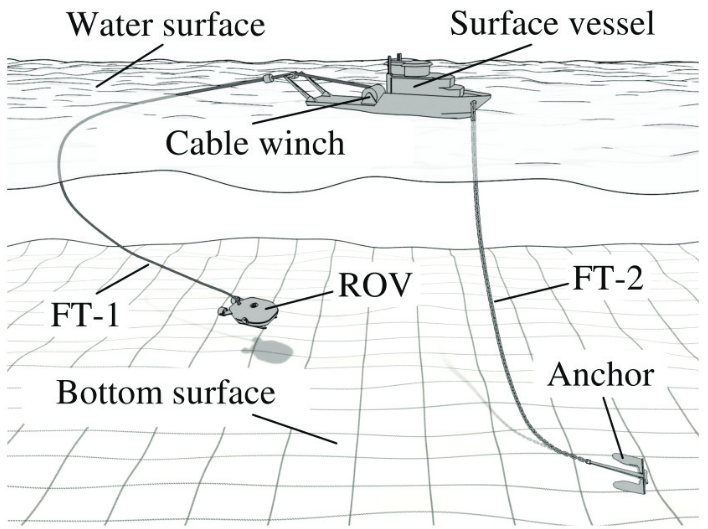
\includegraphics[width=0.4\textwidth]{imgs/underwater_environment.png}
	\caption{Example of a complex underwater environment, \textit{O.  Blintsov,  “Development  of  the  mathematical  modeling  method  for dynamics of the flexible tether as an element of the underwater complex”, 2017}.~\cite{blintsov_development_2017}}
	\label{fig:underwater_environment}
\end{figure}

Most of the existing solutions in terms of physical simulation are position-based simulations~\cite{bender_simulation_methods}. This is a field that is well found in the various references that propose flexible tether simulation methods. The idea is to make a simulation based on a discretization of the tether by finite elements, whose successive positions over time are calculated by a force-based approach~\cite{blintsov_development_2017,marshall,ganoni_unreal, koenemann_modeling_2017, prabhakar_dynamics_2005}.

The problem induced by this method is that it is essential to know the force that each node applies to its neighbor, which is not necessarily known. Some use the equations of continuum mechanics to determine this force~\cite{koenemann_modeling_2017, prabhakar_dynamics_2005}, and others propose a method based on a proportional corrector on the erroneous distance between adjacent nodes~\cite{ganoni_unreal,blintsov_development_2017}.

The idea proposed in this paper is to solve this problem using finite element simulation. This implies that we need to discretize the tether to simulate its global behavior.